% Figure D: the three interventions on a written value, TikZ standalone.
% Encoding: solid boxes = visible token stream (monospace = literal text,
% italic serif = descriptor spans); dashed box = hidden state.
% Colors: vermillion = target value, green = state intervention,
% blue = attention intervention, black = text intervention.
\documentclass[tikz]{standalone}
\usetikzlibrary{positioning,arrows.meta,calc}
\definecolor{okblue}{HTML}{0072B2}
\definecolor{okgreen}{HTML}{009E73}
\definecolor{okverm}{HTML}{D55E00}
\begin{document}
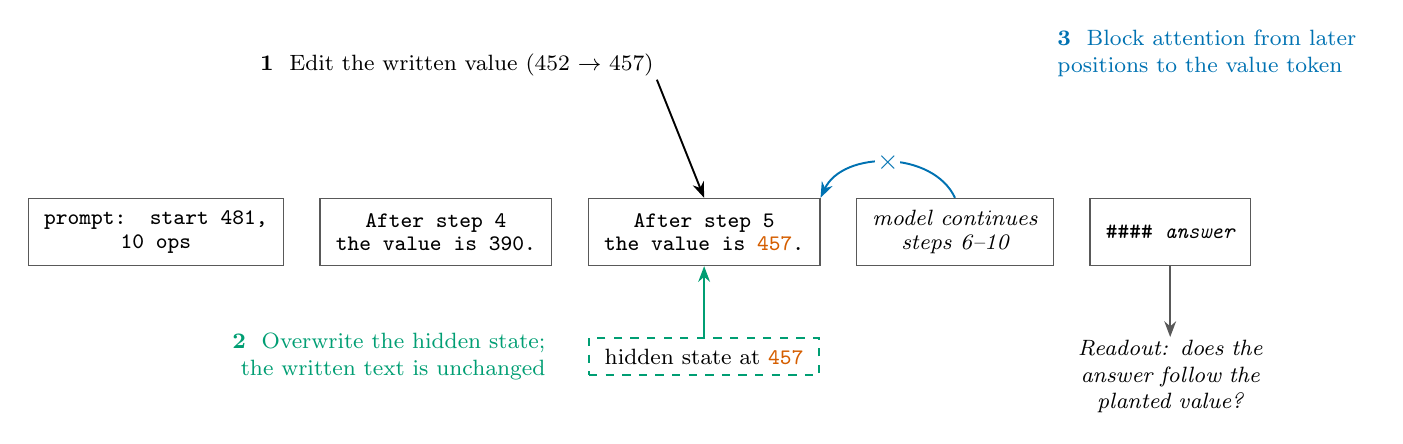
\begin{tikzpicture}[
  font=\footnotesize,
  span/.style={draw=black!65, line width=0.5pt, minimum height=8.5mm,
               inner xsep=2.0mm, inner ysep=1.5mm, align=center},
  hidden/.style={draw=okgreen, dashed, line width=0.6pt,
                 inner xsep=2.0mm, inner ysep=1.4mm, align=center},
  lbl/.style={align=left, inner sep=1pt},
  arr/.style={-{Stealth[length=2.0mm]}, line width=0.7pt},
]
% ---- written token stream ----
\node[span] (p1) {\ttfamily prompt: start 481,\\[-1pt] \ttfamily 10 ops};
\node[span, right=4.5mm of p1] (p2)
  {\ttfamily After step 4\\[-1pt] \ttfamily the value is 390.};
\node[span, right=4.5mm of p2] (p3)
  {\ttfamily After step 5\\[-1pt] \ttfamily the value is \textcolor{okverm}{457}.};
\node[span, right=4.5mm of p3] (p4) {\itshape model continues\\[-1pt] \itshape steps 6--10};
\node[span, right=4.5mm of p4] (p5) {\ttfamily \#\#\#\#~\itshape answer};

% ---- intervention 1: edit the written text ----
\node[lbl, anchor=south east] (i1) at ($(p3.north)+(-6mm,15mm)$)
  {\textbf{1}~~Edit the written value (452 $\to$ 457)};
\draw[arr] (i1.south east) -- (p3.north);

% ---- intervention 2: overwrite the hidden state ----
\node[hidden, below=9mm of p3] (h)
  {hidden state at \textcolor{okverm}{\ttfamily 457}};
\draw[arr, okgreen] (h.north) -- (p3.south);
\node[lbl, anchor=east, okgreen, align=right] (i2)
  at ($(h.west)+(-5mm,0)$)
  {\textbf{2}~~Overwrite the hidden state;\\ the written text is unchanged};

% ---- intervention 3: block attention to the value token ----
\node[lbl, anchor=south west, okblue, text width=40mm] (i3)
  at ($(p4.north east)+(0mm,15mm)$)
  {\textbf{3}~~Block attention from later positions to the value token};
\draw[arr, okblue] (p4.north) to[out=115, in=65]
  node[pos=0.5, fill=white, inner sep=0.6pt, font=\normalsize] {$\times$}
  (p3.north east);

% ---- readout ----
\node[lbl, below=9mm of p5, align=center, text width=30mm] (ro)
  {\itshape Readout: does the answer follow the planted value?};
\draw[arr, black!65] (p5.south) -- (ro.north);
\end{tikzpicture}
\end{document}
